% Uncomment this line for on-screen presentation
\documentclass[xcolor={dvipsnames}]{beamer}\usepackage{etoolbox}\newtoggle{printable}\togglefalse{printable}

% Uncomment this line for printable slides (disable animations and don't waste ink)
%\documentclass[handout, xcolor={dvipsnames}]{beamer}\usepackage{etoolbox}\newtoggle{printable}\toggletrue{printable}

% Adjust these for the path of the theme and its graphics, relative to this file
%\usepackage{beamerthemeFalmouthGamesAcademy}
\usepackage{../../beamerthemeFalmouthGamesAcademy}
\graphicspath{ {../../} }

% Default language for code listings
\lstset{language=C++,
		morekeywords={each,in}
}

\begin{document}
\title{Programming Practice I}   
\subtitle{BSc Computing for Games}

\frame{\titlepage} 

\part{Morning}
\frame{\partpage}

\begin{frame}{Game Design}
	In the morning session you will:
	
	\begin{itemize}
		\item \textbf{Self-organise} into \textbf{TWO} groups of approximately equal size.
		\item \textbf{Design} a short text-based adventure game with the following themes:
		\begin{itemize}
			\item Group wearing the \textit{most red}: ``Iron Bull''.
			\item Group wearing the \textit{least red}: ``Ghostly Spymaster''.
		\end{itemize}
	\end{itemize}
\end{frame}

\begin{frame}{Game Design}
	\begin{itemize}
		\item Reflect upon Monday’s COMP140 lecture activity as well as the associated reading material 
		to distil the key elements that form the design and how to describe them
		\item Research what is usually included in a game design document to help guide your design 
		process. Start here:
		\begin{itemize}
			\item \url{http://www.gamasutra.com/view/feature/131791/the_anatomy_of_a_design_document_.php}
			\item \url{http://www.gamasutra.com/view/feature/130127/design_document_play_with_fire.php}
		\end{itemize}
	\end{itemize}
\end{frame}

\part{Afternoon}
\frame{\partpage}

\begin{frame}{Game Design}
	In the afternoon session you will:
	
	\begin{itemize}
		\item \textbf{Create} a rough prototype of the mechanic associated with conflict.
		\begin{itemize}
			\item Start out with a low-fidelity paper prototype.
			\item If making a digital prototype, apply pair programming and use whichever tools
			and programming language that you deem most appropriate.
		\end{itemize}
		\item \textbf{Prepare} a 30-second ``elevator'' pitch.
		\item \textbf{Prepare} to demonstrate your prototypes to the tutor.
	\end{itemize}
\end{frame}

\begin{frame}{Game Design}
	\begin{itemize}
		\item Avoid over-scope! This is a tiny project!
		\item The prototype does not need to be fully functional. It should be used as a communication tool to demonstrate the design ideas.
		\item Do not worry about the pitch or what should be included in it. Aim to only include those things that help you communicate 
		your design ideas. This is not an assessment, but an opportunity to reflect and practice.
	\end{itemize}
\end{frame}

% -------------------------------------------------------

%\part{The compiler}
%\frame{\partpage}
%
%\begin{frame}
%	\frametitle{The build process}
%	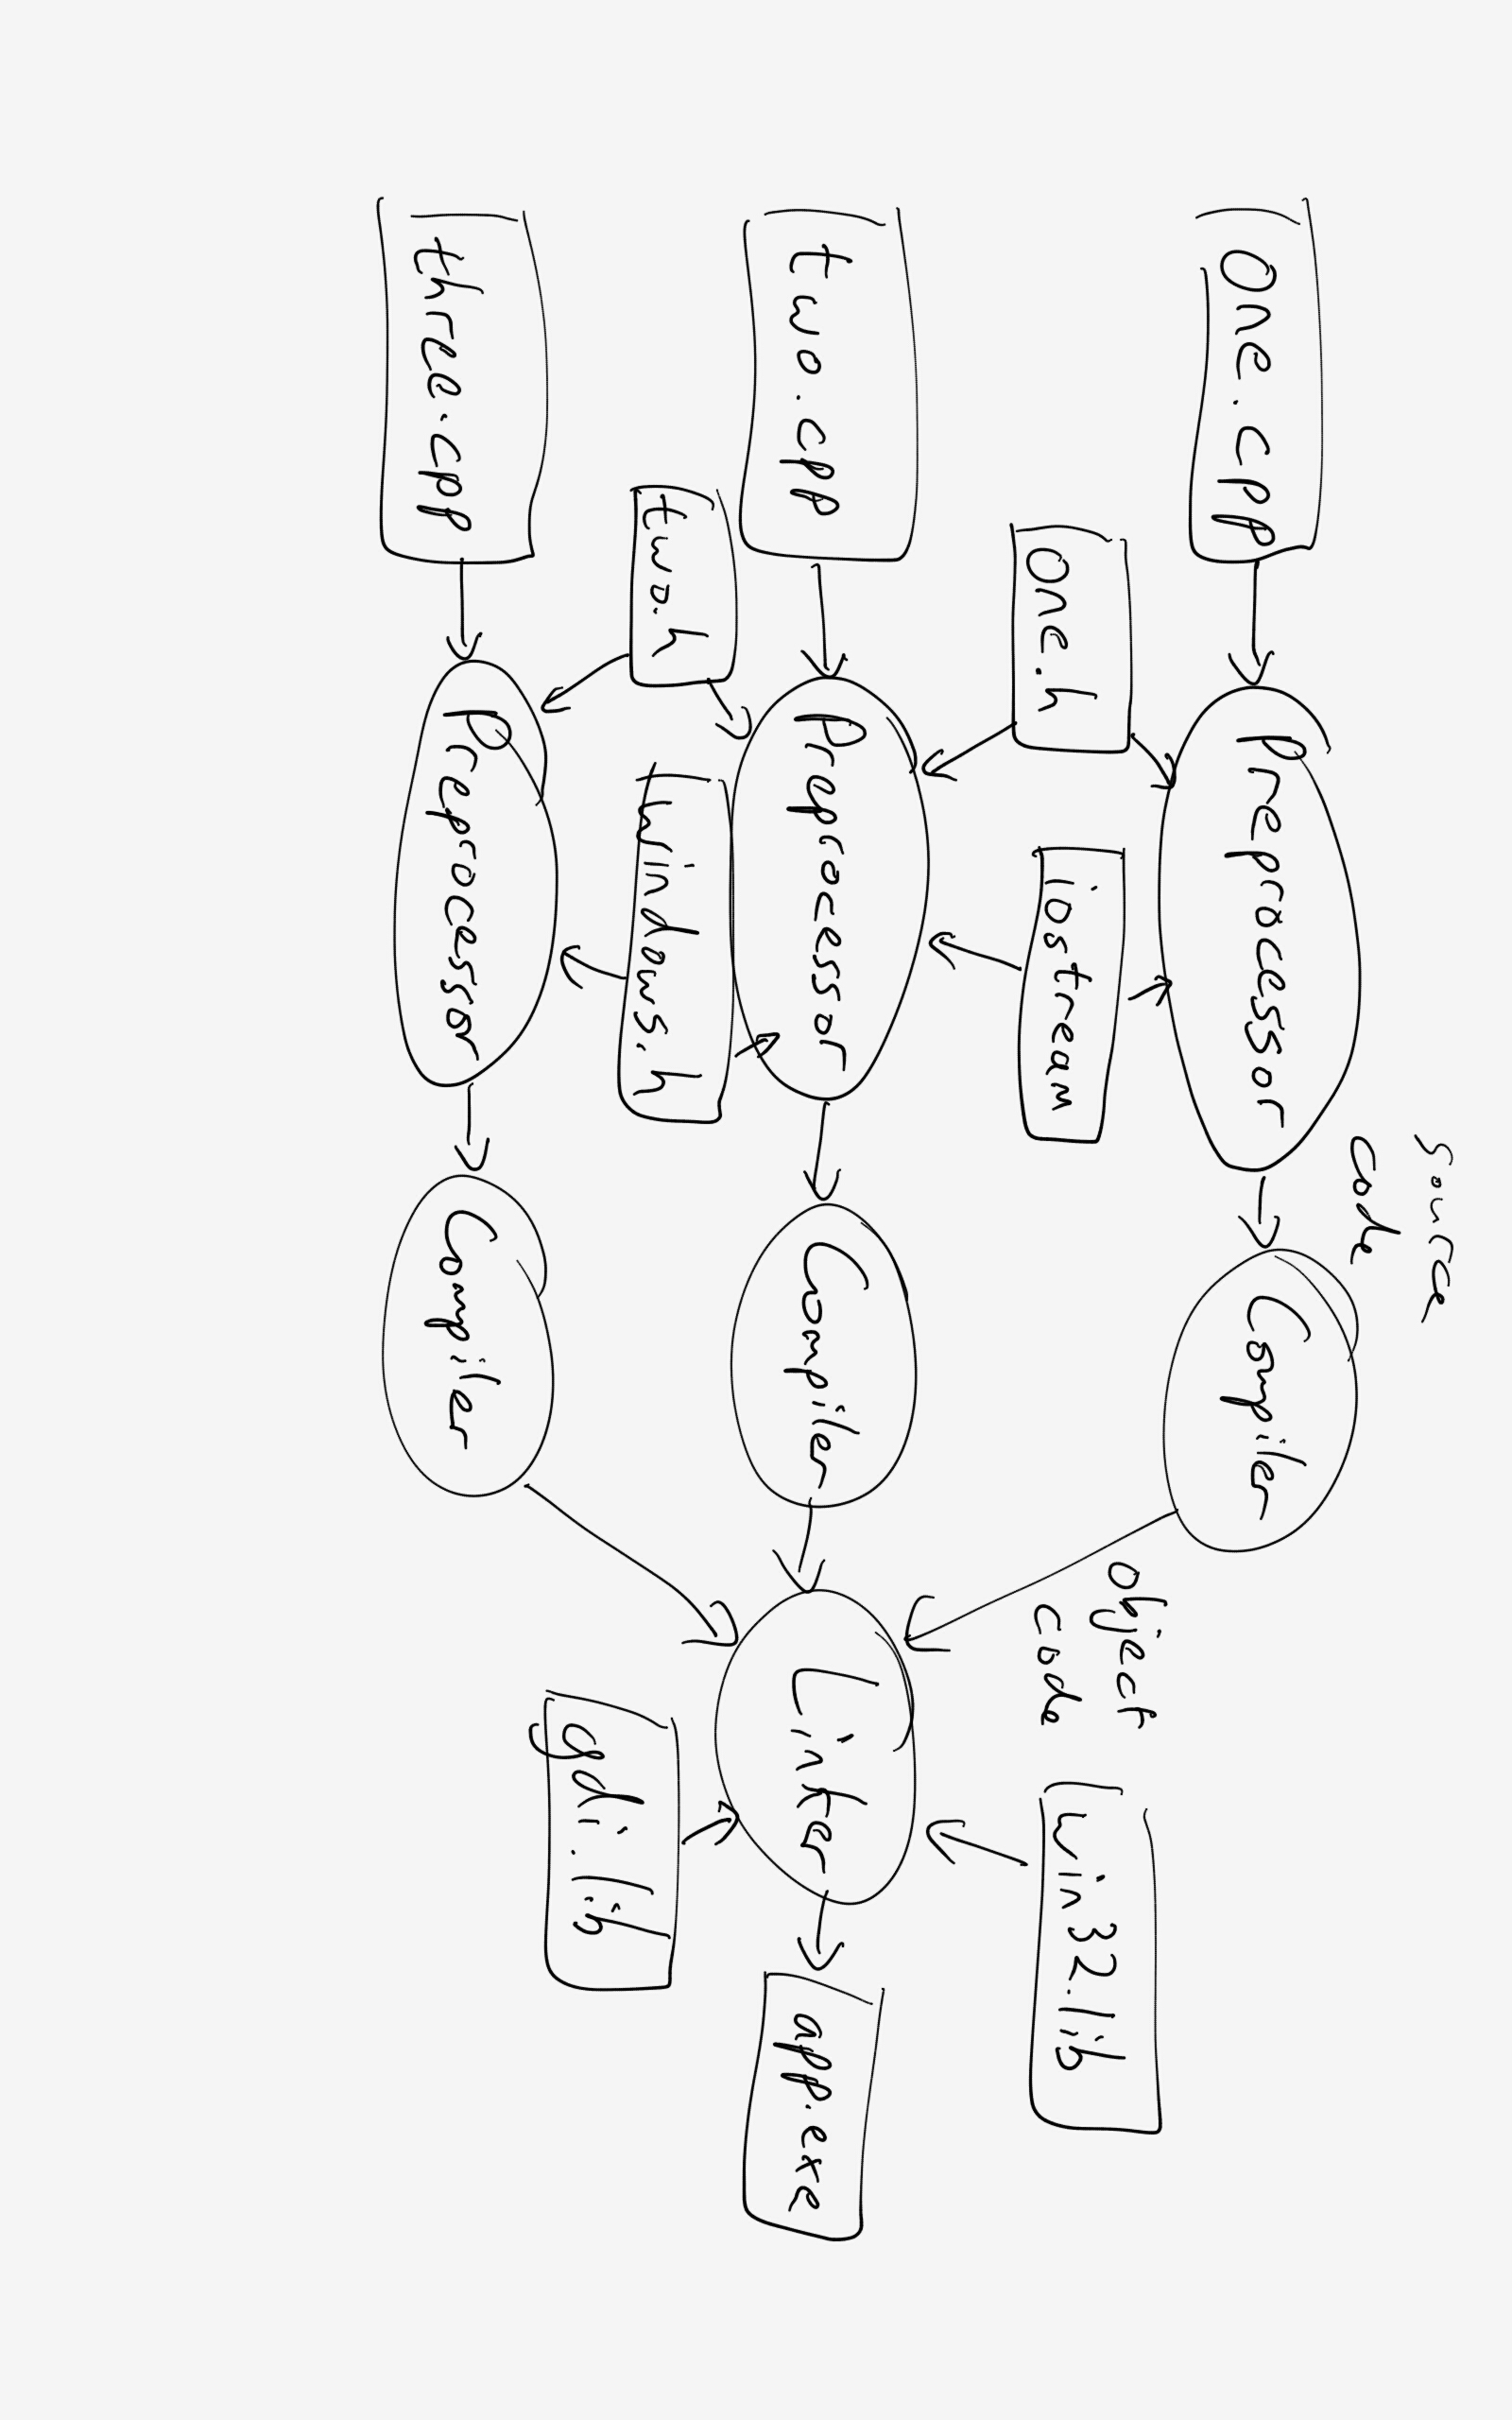
\includegraphics[height=\textwidth,angle=90]{compiler_sketch}
%\end{frame}

\end{document}
